%\documentclass[sigconf]{acmart}

\documentclass{vldb}

%\usepackage{balance}  % for  \balance command ON LAST PAGE  (only there!)


% Include information below and uncomment for camera ready
%\vldbTitle{Optimization of Machine Learning Workloads with Experiment Databases}
%\vldbAuthors{Behrouz Derakhshan, Alireza Rezaei Mahdiraji, Tilmann Rabl, and Volker Markl}
%\vldbDOI{https://doi.org/10.14778/xxxxxxx.xxxxxxx}
%\vldbVolume{xx}
%\vldbNumber{xxx}
%\vldbYear{2020}

\vldbTitle{}
\vldbAuthors{}
\vldbDOI{}
\vldbVolume{}
\vldbNumber{}
\vldbYear{}

%\settopmatter{printacmref=false} % Removes citation information below abstract
%\renewcommand\footnotetextcopyrightpermission[1]{} % removes footnote with conference information in first column
%\pagestyle{plain}

\usepackage{mathtools}
%\usepackage{array}
\usepackage{url}
\usepackage{lmodern}
%\usepackage[export]{adjustbox}
%\usepackage{lipsum}% http://ctan.org/pkg/lipsum
%\usepackage{graphicx}% http://ctan.org/pkg/graphicx
%\usepackage{soul}
\usepackage{xcolor}
% Use hladd to highlight newly added text
\newcommand\hladd[1]{%
  \bgroup
  \hskip0pt\color{blue}%
  #1%
  \egroup
}

% Use hldel to highlight text that will be removed
\newcommand\hldel[1]{%
  \bgroup
  \hskip0pt\color{red!80!black}%
  #1%
  \egroup
}
% Use hl when the highlighted text should be discussed with a reviewer (marked in the .tex file)
\newcommand\hl[1]{%
  \bgroup
  \hskip0pt\color{green!80!black}%
  #1%
  \egroup
}
%\usepackage{float}
%\usepackage{amsmath}
\usepackage{todonotes}
\usepackage{subcaption}
\usepackage[outdir=./figures/]{epstopdf}
\usepackage{listings}
%\usepackage{booktabs}
%\usepackage{upquote}
\usepackage{makecell}
%\usepackage{courier}
%\usepackage[scaled]{beramono}

%\usepackage[linesnumbered,ruled,vlined]{algorithm2e}
\usepackage{algorithm}% http://ctan.org/pkg/algorithms
\usepackage[noend]{algpseudocode}% http://ctan.org/pkg/algorithmicx

% command for drawing a circle around text  
\newcommand{\circledtext} [1] {\raisebox{.5pt}{\textcircled{\raisebox{-.9pt} {#1}}}}

\algrenewcommand\algorithmicrequire{\textbf{Input:}}
\algrenewcommand\algorithmicensure{\textbf{Output:}}
\algdef{SE}[DOWHILE]{Do}{DoWhile}{\algorithmicdo}[1]{\algorithmicwhile\ #1}%

\definecolor{forestgreen}{rgb}{0.13, 0.55, 0.13}
\lstdefinestyle{pythonstle}{
language=Python,
basicstyle=\scriptsize\ttfamily,
columns=fullflexible,
numbers=left,
stepnumber=1,
numbersep=5pt,
xleftmargin=10pt,
frame=single,
framexleftmargin=3pt,
otherkeywords={self},             % Add keywords here
keywordstyle=\color{forestgreen},
emph={MyClass,__init__},          % Custom highlighting
emphstyle=\color{red},    % Custom highlighting style
stringstyle=\color{blue},
frame=tb,                         % Any extra options here
showstringspaces=false        % 
}
\lstset{style=pythonstle}

\PassOptionsToPackage{table}{colorx}
%\usepackage[utf8]{inputenc}
%\usepackage{pgfplots}
\DeclareMathOperator*{\argmin}{arg\,min}
\DeclareMathOperator*{\argmax}{argmax}
% ACM Reference and Copy right
%\settopmatter{printacmref=false}
%\makeatletter
%\def\@copyrightspace{\relax}
%\makeatother

\begin{document}
%\lstset{numbers=left, numberstyle=\small, numbersep=8pt, frame = single, language=Pascal, framexleftmargin=15pt}

\title{Optimization of Machine Learning Workloads in Collaborative Data Science Platforms}

%
% You need the command \numberofauthors to handle the 'placement
% and alignment' of the authors beneath the title.
%
% For aesthetic reasons, we recommend 'three authors at a time'
% i.e. three 'name/affiliation blocks' be placed beneath the title.
%
% NOTE: You are NOT restricted in how many 'rows' of
% "name/affiliations" may appear. We just ask that you restrict
% the number of 'columns' to three.
%
% Because of the available 'opening page real-estate'
% we ask you to refrain from putting more than six authors
% (two rows with three columns) beneath the article title.
% More than six makes the first-page appear very cluttered indeed.
%
% Use the \alignauthor commands to handle the names
% and affiliations for an 'aesthetic maximum' of six authors.
% Add names, affiliations, addresses for
% the seventh etc. author(s) as the argument for the
% \additionalauthors command.
% These 'additional authors' will be output/set for you
% without further effort on your part as the last section in
% the body of your article BEFORE References or any 
%\author{
%{\large Behrouz Derakhshan, Alireza Rezaei Mahdiraji, Tilmann Rabl, and Volker Markl}\\
%\affaddr{}\\
%\affaddr{ $ $ DFKI GmbH       \hspace{2.2cm}     Technische Universität Berlin}\\
%\affaddr{ \{behrouz.derakhshan, alireza.rm, tilmann.rabl, volker.markl\}@dfki.de} 
%}


\maketitle
\begin{abstract}
\hladd{Collaborative data science platforms, such as Google Colaboratory and Kaggle, affected the way users solve machine learning tasks.
Instead of solving a task in isolation, users write their machine learning workloads and execute them on these platforms and share the workloads with others.
This enables new users to learn from and modify existing workloads, which will ultimately lead to more efficient solutions for solving the task.
As a result, many executed operations in collaborative platforms, especially the data preprocessing operations, are repeatedly executed by different users.
However, current collaborative platforms only store scripts, raw training datasets, and in some cases the final machine learning models and ignore any intermediate artifacts such as preprocessed and cleaned data.
As a result, the platforms miss an opportunity for improving the execution time of future machine learning workloads.
%First, storing all the artifacts, , requires massive amounts of storage.
%As a result, only some of the artifacts such as raw data and machine learning models are stored and users must re-execute the scripts and operations to reconstruct the desired artifact.
%\hl{Second, even if all the artifacts are stored, manually finding desired artifacts is a time-consuming process.} % Tilmann: this is only a conclusion of the first problem, better say finding the artifacts is slow or similar... *Behrouz: I wanted to use the word manually (or something equal) to contrast between the current 'manual' querying or reading the scripts vs our way of reuse or warmstarting that doesn't require user's intervention.

The contributions of this paper are two-fold.
First, we utilize a graph to store the artifacts and operations of machine learning workloads as vertices and edges, which we refer to as the experiment graph.
Since storing all the artifacts is not feasible, as the size of the intermediate artifacts may grow exponentially, we propose two algorithms for materializing the artifacts with high likelihoods of future reuse.
The algorithms consider several metrics, such as access frequency, size of the artifact, and quality of machine learning models to decide what artifacts to materialize.
Second, using the experiment graph, we propose a novel approach for quickly finding artifacts to reuse or to warmstart model training operations in future workloads.}
%TODO one sentence the impact

%Machine learning workloads have varying characteristics.
%Some involve a large user base where a combination of experts and novice users are trying to design machine learning pipelines and execute them on specific tasks, such as online education, data science challenges.
%Some involve fewer users, typically experts, working together to solve a task.
%For example, a team of data scientists in a company trying to design a recommender system based on the available training data.
%Both workloads are interactive and require many iterations to improve the solution.
%In such scenarios, communication between the users involved is not optimal and as a result, many repetitions may occur.
%Repetitions can be of the form of repeated data preprocessing, hyperparameter search, and model training.
%
%Using experiment databases, where a log of previous machine learning experiments is stored, we propose a solution that utilizes the information in the experiment database to improve the process of design and execution of machine learning workloads.
%Specifically, we utilize the logs in the experiment databases to reduce the data processing and model training time by caching and reusing the preprocessed data and trained models.
%Moreover, we leverage the logs to enhance the hyperparameter optimization process and provide the users (both expert and novice) with better hyperparameter settings in a shorter amount of time.
\end{abstract}
%\keywords{Machine Learning Model Management; End to End Machine Learning; Experiment Databases}

\section{Introduction} \label{sec-introduction}
% Opening
Machine learning is at the core of academic and industry.
To make sense of the data, one designs a machine learning pipeline, selects training algorithm, finds appropriate parameters (typically called hyperparameters), and finally utilize the pipeline to solve a task.
The space of available tools, data preprocessing methods, training algorithms, and their parameters is typically large.
This overwhelms expert data scientist, let alone novice users.

% G
Recently, the scientific community embraced collaborative science to improve the work.
By storing logs of machine learning experiments which includes information about the data, the algorithms and their parameters, and the results in a structured way, data scientists can share information.
By sharing information, users can learn from other users work.
% P
However, the abundance of information still overwhelms users.
As a result, searching through the experiment database to find how others have solved similar tasks or what is the result of specific data operation or machine learning algorithm on a dataset creates more overhead than if the data scientist executes their hypothesis and see the result for themselves.
% S
Our solution is to utilize established database optimization techniques (such as view materialization and caching) and novel optimization strategies to enhance the user experience by automatically optimize the given workload.

We identify two groups of audiences typically utilize a machine learning system: expert data scientists and novice users.
Each group have different mode of operation when designing and executing machine learning models for solving tasks.
The expert scientists typically first analyze the data by computing several statistics.
Based on the initial analysis they form hypothesis which leads to the creation of a machine learning pipeline and a training algorithm.
Moreover, they also have a good understanding of each component therefore, they rely on grid search methods to try out many different set of hyperparameters.
On the other hand, novice users have less knowledge and they would like to try out different models.
They would like to be given hints on what are the good data preprocessing steps, training algorithms, and hyperparameters to apply to the given dataset.

Our key idea is to leverage the experiment database to speed up the data processing and grid search for expert users and use the knowledge of the expert users to enhance the experience of the novice users.
The initial analysis of expert users are typically involve many similar steps.
Moreover, the grid that they specify for searching through hyperparameters typically have overlapping branches with other experts.
By analyzing the meta-data of the existing experiments we can determine the frequent transformations and cache them.
This can save time by skipping many of the data operation of the subsequent users.
Moreover, after defining a grid search, we utilize the experiment database to inform the user on the branches that are already computed and provide the result without recomputing them.
\section{Background} \label{sec-background}
In this section, we first define the required terms referring to different entities in collaborative environments which we use throughout the paper.
Next, we discuss a use case based on a real collaborative environment.

\subsection{Collaborative Environment for Data Science}
A typical collaborative environment consists of a client and server space.
Users write a script to fetch datasets from the server, analyze the data, and train machine learning models.
The client is responsible for executing the script.
Although the client can be a single machine, users typically utilize Jupyter notebooks  \cite{Kluyver:2016aa} to write and execute their scripts in isolated containers \cite{merkel2014docker} within the server itself \cite{kagglewebsite, googlecolab, netflix-notebook}.
Users can publish the results and the scripts on the server for other users to see.
Isolated execution environments enable collaborative environments to better allocate resources for running scripts.

%\subsection{Preliminaries and Definitions}
%\textbf{ML Task.} 
%In a collaborative environment, an ML task specifies the requirements and the goal of the machine learning solutions.
%An ML task contains the following: (1) The type of the machine learning model, i.e., classification, regression, or clustering, (2) one or more training and test datasets, and (3) an evaluation function which assigns a score to the user-provided solution.
%For example, in an online advertising company, the ML task for the data scientists is to train Click-Through-Rate prediction models given one or multiple datasets containing users and ads features which minimize the logarithmic loss on a test dataset.
%
%\textbf{Data and Operations.}
%We support three types of data: (1) A \textit{Dataset} which has one or more columns of data and is analogous to dataframe objects, such as Pandas dataframe \cite{mckinney-proc-scipy-2010}), (2) an \textit{Aggregate} which contains a single value or list of values, and (3) a \textit{Model} which represents a machine learning model.
%The type of data depends on the operations which generate them.
%\textit{Data preprocessing and feature engineering operations}, which include simple data transformation and aggregation, feature selection, and feature extraction operations, generate either a Dataset (e.g., map, filter, or one-hot encoding operations)  or an Aggregate (e.g., reduce operation).
%\textit{Model training operations} generate a Model.
%A Model is used either in other feature engineering operations, e.g., PCA model for dimensionality reduction, or to perform predictions on a test dataset.
% 
%\textbf{ML Workload.}
%An ML workload is a script or a machine learning pipeline which performs several data preprocessing, feature engineering, and model training operations. 
%Collaborative platforms execute a workload in either a long-running process or an interactive environment using Jupyter notebooks \cite{Kluyver:2016aa}.

\subsection{Use Case}\label{subsec-motivational-example}
Kaggle is a collaborative environment that enables users and organizations to publish datasets and organize machine learning competitions by defining a task where all the users can participate and submit workloads for solving the task \cite{kagglewebsite}.
Kaggle utilizes docker containers, which are called kernels, to execute user workloads.
If the workload produces machine learning model artifacts, the users can choose to submit them and attain a score of how good their model performs on a test dataset.

For our use case, we select the competition \textit{Home Credit Default Risk}\footnote{https://www.kaggle.com/c/home-credit-default-risk/}.
The task is to train a classification model to predict whether a client can repay their loans.
There are a total of 9 datasets, 8 for training and 1 for evaluation, with a total size of 2.5 GB.
The goal of the submitted workloads is to produce machine learning models which maximize the area under the ROC curve, which measures how well a classifier performs.
Three of the most popular submitted workloads are copied and edited by different users more than 7000 times\footnote{Notebook titles are: ''Start Here: A Gentle Introduction'' and ''Introduction to Manual Feature Engineering'' part 1 and part 2}.
The three workloads produce 100s of intermediate dataset artifacts and several machine learning model artifacts with a total size of 125 GB.
The execution time of each workload is between 400 to 1000 seconds.
Kaggle does not provide any information on the number of workload executions.
However, the number of users who copied these workloads indicates the potentially large number of executions, i.e., at least 7000 times.

Kaggle does not store the artifacts, nor does it offer any automatic reuse capabilities.
Therefore, every time a user executes these workloads (or a modified version of them), Kaggle runs them from scratch.
Our system, which stores the artifacts and reuses them later, can save 100s of hours of execution time only for the three workloads in this use case, which benefits Kaggle by reducing the amount of required resources and operation cost.
In the next sections, we show how we selectively store artifacts, given a storage budget, and how we quickly find the relevant artifacts for reuse.
\section{ML Workload Optimizations} \label{sec-ml-workloads}
In this section, we first describe the common types of operations in machine learning workloads.
Then, we discuss how to capture and store the operations in the experiment graph.
Lastly, we discuss how do we utilize the experiment graph to optimize new workloads.

\subsection{Operations in ML Workloads}
We assume the main units of work are dataframe (e.g., Pandas, R Data Frames, and Spark DataFrames) like objects that contain one or many columns, where all the data items in one column are of the same data type.
\hl{We divide the operations in the ML workloads into 3 categories.}
\begin{table}
\centering
\begin{tabular}{ll}
\hline
	   Feature Extraction & Feature Selection\\ \hline
        feature hasher & variance threshold  \\
        one hot encoding & select k best \\
        count vectorizer& select percentile \\ 
        tfidf transformer & recursive feature elimination \\
        hashing vectorizer & select from model \\
        extract\_patch\_2d &  \\
        \hline
\end{tabular}
\caption{List of feature extraction and feature selection operations}\label{feature-engineering-operations}
\end{table}

\subsubsection{Data and Feature Engineering}
This group of operations typically belongs to three categories, i.e., simple data transformations and aggregations, feature selection, and feature extraction.
All of these operations, receive one or multiple columns of a dataset and return another dataset as result. 
While different data processing tools may provide specialized data transformation and aggregation operations for dataframe objects, most of them provide the same or similar operations such as map, reduce, group by, concatenation, and join. 
In Table \ref{feature-engineering-operations}, we show a list of the most common feature extraction and feature selection operations.

\subsubsection{Model Training}
Model training operations are a group of operations that receive a dataset (or one or multiple columns of a dataset) and return a machine learning model.
The result of model training operations can either be used in other data and feature engineering operations (e.g., applying PCA to reduce the number of dimensions of the data) or can be used to perform prediction (for classification and regression tasks) on unseen data.

\subsubsection{Hyperparameter Tuning}
Before training a machine learning model, one has to set the hyperparameters of the model to appropriate values.
Typically, the best values for the hyperparameters of a model vary across different datasets.
The goal of hyperparameter tuning operations is to find the machine learning models with the best performance.
A hyperparameter tuning operation is defined by a budget and a search method.
The budget specifies how many models with different hyperparameter values the operation should train and the search method specifies what search strategy should be incorporated.
We limit our focus to popular search methods, namely, grid search, random search, and Bayesian hyperparameter search \cite{bergstra2012random,snoek2012practical}.

\subsection{Experiment Graph Representation}\label{sub-graph-construction}
To efficiently apply our optimizations, we utilize a graph data structure, called the experiment graph, to store the meta-data and artifacts of the machine learning workloads.
Let $\mathcal{V}=\{v_i\}, i = 1, \cdots, n$ be a collection of artifacts that exist in the workload.
Each artifact is either a raw dataset, a pre-processed dataset resulting from a feature engineering operation, or a model resulting from a model training operation.
Let $\mathcal{E}=\{e_i\}, i = 1, \cdots, m$ be a collection of executed operations that exist in the workload.
A directed edge $e$ from $v_i$ to $v_j$ in $\mathcal{G}(\mathcal{V},\mathcal{E})$ indicates that the artifact $v_j$ is (fully or partially) derived from the artifact $v_i$ by applying the operation in $e$.
Every vertex $v$ has the attribute $\langle s \rangle$ (accessed by $v.s$), which represents the storage size of artifact when materialized.
Every edge $e$ has the attributes $\langle f, t\rangle$ (accessed by $e.f$ and $e.t$), where $f$ represents the frequency of the operation (the number of times the operation has been executed) and $t$ represents the average run-time (in seconds) of the operation.
Each vertex contains meta-data about the artifacts, such as the name and type of the columns for datasets and name, size, the value of parameters and hyperparameters, and the error metric of the models.
Each edge contains the meta-data about the operation, such as the function name, training algorithm, hyperparameters, and in some cases even the source code of the operation.
When a new machine learning workload is executed, we extend the graph to capture the new operations and artifacts.
If an operation already exists in the graph, we update the frequency and average run-time attributes.
Otherwise, we add a new edge and vertex to the experiment graph, representing the new operation and the artifact.
Figure \ref{fig-experiment-graph}a shows an example graph constructed from the code in Listing \ref{listing-experiment-graph}.
To uniquely identify an edge, we utilize a hash function that receives as input the operation and its hyperparameters (if it has any).

\begin{lstlisting}[language=Python, caption=Example script,captionpos=b,label = {listing-experiment-graph}]
import numpy as np
import pandas as pd

from sklearn import svm
from sklearn.feature_selection import SelectKBest
from sklearn.feature_extraction.text import CountVectorizer

train = pd.read_csv('../input/train.csv') 
print train.columns # [ad_desc,ts,u_id,price,y]
vectorizer = CountVectorizer()
count_vectorized = vectorizer.fit_transform(train['ad_desc'])
selector =  SelectKBest(k=2)
top_features = selector.fit_transform(train[['ts','u_id','price']], 
				      train['y'])
X = pd.concat([count_vectorized,top_features], axis = 1)
model = svm.SVC()
model.fit(X, train['y'])
\end{lstlisting}

\begin{figure}
\begin{subfigure}[b]{0.4\linewidth}
\centering
\documentclass{standalone}
\usepackage{tikz}
\usetikzlibrary{graphdrawing, graphs, quotes, positioning,arrows, backgrounds, math, calc, shapes, positioning}
\usegdlibrary{trees}
\begin{document}
\begin{tikzpicture}
%\draw[help lines]  (-2,0) grid (6,6);
\tikzstyle{every node}=[inner sep=0.02cm]
\node (train) [ellipse, draw] at (2,6) {$train$};
% layer 1
\node (ad) [ellipse, draw, below left = of train] {$ad\_desc$};
\node (forselection) [ellipse, draw, below = of train] {$t\_subset$};
\node (y) [ellipse, draw, below right = of train] {$y$};
% layer 2
\node (cv) [ellipse, draw, below = of ad] {$cnt\_vect$};
\node(sk) [ellipse, draw, below = of forselection] {$top\_features$};
% layer 3
%\node (merged1) [circle, draw] at (1.5, 3.5) {$v_6$};
\node (cvsk) [ellipse, draw, below = of sk] {$X$};
% layer 4
%\node(merged2) [circle, draw] at (3, 2.8) {$v_8$};
% layer 5
\node(model) [ellipse, draw, below right = of cvsk]  {$model$};

\graph [grow down,edge quotes ={inner sep=1pt}, edges ={thick},radius=.2cm, nodes={circle, draw,font =\small}]{
(train) [label=train]
-> [anchor=east, align=center,"p1"] (ad)
-> [anchor=east,align=center,"vf1"] (cv)
%-> [anchor=east,align=center,"m"](merged1) 
-> [anchor=east,align=center,"c1"](cvsk) 
%-> [anchor=south, align=center,"m"](merged2) ;
-> [anchor=east,auto=false,align=center,"f"] (model);

(train) 
-> [anchor=east,align=center, "p2"] (forselection)
-> [anchor=east,auto=false,align=center,"s1"] (sk)
-> [anchor=east,align=center,"c1"](cvsk) ;

(train) 
-> [anchor=west, align=center,"p3"]   (y)
%-> [anchor=west, align=center,"m"](merged2) 
-> [anchor=east,auto=false,align=center,"f"] (model);
};
\end{tikzpicture}
\end{document}
\caption{}
\end{subfigure}%
\begin{subfigure}[b]{0.6\linewidth}
\begin{tabular}{lcl}
\hline
operation & label &  hash \\
\hline
project(ad..) & $\langle 2, 2\rangle$ &p1 \\
project(ts, ..) & $\langle 1, 6\rangle$ & p2\\
project(y) & $\langle 1, 2\rangle$ & p3\\
vectorizer.f\_t & $\langle 2, 40\rangle$ & v1 \\
selector.f\_t & $\langle 1, 60\rangle$ & s1 \\
concat & $\langle 1, 10\rangle$ & c1 \\
merge & $\langle 1, 0 \rangle$ & m\\
model.fit & $\langle 1, 100\rangle$ & f\\
\hline
\end{tabular}
\caption{}
\end{subfigure}
\caption{Experiment graph constructed from the Listing \ref{listing-experiment-graph} (a) and the hash of the operations in the scripts (b)}
\label{fig-experiment-graph}
\end{figure}
Table \ref{fig-experiment-graph}b shows both the label of every edge operation, i.e., frequency and time, and the hash of the operations and their hyperparameters.
We assume the operations project(ad..) and vectorizer.f\_t already exist in the experiment graph.
Therefore, when adding the new operations, we must update their frequency to 2.
In order to represent operations that process multiple input artifacts, e.g., concat and model.fit operations in Listing \ref{listing-experiment-graph}, we proceed as follows.
First, we merge the vertices representing the artifacts into a single vertex using a merge operator.
The merge operator is a logical operator which does not incur a cost, i.e., it has run-time of 0 seconds.
The merged vertex is also a logical vertex with no actual attributes which only contains the vertex id of the merged vertices.
Then, we draw an edge from the merged vertex which represents the actual operation.
For example, in Figure \ref{fig-experiment-graph}a, before applying the concatenation operation, we merge $v_4$ and $v_5$ into $v_6$, then we apply the concatenation operation (c1).
This is a critical step for the materialization algorithms and optimization strategies.

%It is important to note that based our definition of a task in Section \ref{sec-introduction}, the workloads belong to multiple different tasks, the constructed graph will contain one connected component for every task.
%In the next sections, we assume that the experiment graph contains information about 1 task, although, all the methods described can be applied to multiple tasks as well.
\subsection{Workload Optimizer for Kaggle Use Case}
By utilizing an experiment graph, we can improve the execution of the kernels in Kaggle.
This results in faster execution of the kernels and less time spent in the queue.

Figure \ref{improved-use-case} shows how we utilize the experiment graph in the Kaggle Infrastructure. 
The workflow is as follows.
First, we parse a workload (i.e., a kernel) and construct the workload graph.
Then, an \textbf{optimizer} component receives the workload graph and utilizes the existing experiment graph and look for optimization opportunities, namely, reusing the existing operations, warm starting the model training, and for workloads that contain a hyperparameter tuning operation, an improved tuning.
The result of the optimization is another workload graph which contains precomputed artifacts, warmstarted models, and proper search space and/or an initialized Bayesian hyperparameter search process.
After executing the optimized workload, we return the result to the user.
After the execution, we update the experiment graph using original workload graph.
Finally, to ensure the we can store the experiment graph given our storage limit, we run our materialization algorithms to decide what artifacts to materialize and what artifacts to remove.

\begin{figure}
\centering
\includegraphics[width=\columnwidth]{../images/kaggle-workload-optimizer}
\caption{Improving the execution of Kaggle Kernels with Workload Optimizer}
\label{improved-use-case}
\end{figure}

It is important to note that we restrict the scope of our optimizations and materialization algorithms to one machine learning task. 
In Kaggle, each competition defines the machine learning task, i.e., one or multiple raw training datasets, a validation data set, and an evaluation function which computes the quality/error rate of the model on the validation dataset.
While the experiment graph contains artifacts from all the tasks, each task corresponds to a unique connected component of the experiment graph.
All the artifacts in a task's connected component are reachable from the raw training datasets defined in the task.
When optimizing a new workload (i.e., a Kaggle kernel), we only utilize the connected component the task the workload is trying to solve (i.e., the Kaggle competition) and do not utilize the rest of the graph for optimization.


\section{Artifact Materialization}\label{sec-materialization}
\todo[inline]{Describe the need for materialization, move it from \ref{subsec-ml-based-materialization} and then mention the two algorithms ml-based and storage-aware}
\subsection{ML-Based Materialization}\label{subsec-ml-based-materialization}
Depending on the number of the executed workloads, the generated artifacts may require a large amount of storage space.
For example, in the Home Credit Default Risk Kaggle competition\footnote{https://www.kaggle.com/c/home-credit-default-risk}, one of the popular scripts that analyzes a dataset of 150 MB, generates up to 17 GB of artifacts.
Therefore, materializing every artifact under limited storage is not feasible.
In this section, we discuss our algorithm for materializing a subset of the artifacts under limited storage, a modified version of the algorithm presented by Bhattacherjee et al. \cite{bhattacherjee2015principles}.
The goal of the algorithm is to materialize the artifacts that result in the lowest weighted recreation cost while ensuring the total size of the materialized artifacts does not exceed the storage capacity.
We define $WC$ as the function that computes the weighted recreation cost of the graph $\mathcal{G}$, given the set of materialized vertices $\mathcal{MV}$, where  
\[
WC(\mathcal{G}, \mathcal{MV}) =  \sum\limits_{e \in \{e' \in \mathcal{E}  \lvert dest(e') \notin \mathcal{MV}\}}  e.f \times e.t
\]
and $dest(e)$ represents the destination vertex of the edge $e$.
The weighted recreation cost indicates how much time do we need to spend to execute all the operations, taking into account the repeated executions, in the graph.
For un-materialized artifacts, we must consider the frequency of the operations that produce the artifact.
For example, in Figure \ref{fig-experiment-graph}, if we do not materialize $v_4$ and the operation \textit{vectorizer.f\_t} has a frequency of 2, we must consider both executions of the operation when computing the weighted cost.
Whereas, if $v_4$ is materialized, the \textit{vectorizer.f\_t} operation has no impact on the weighted recreation cost.
%\todo[inline]{show that it is NP hard and cite \cite{bhattacherjee2015principles} and state the differences in their work and solution and ours}
%Bhattacherjee et al. \cite{bhattacherjee2015principles} tackle a similar problem and prove that the problem is NP-hard.
%They provide a greedy solution for the problem as well.
%However, there differences in both the use cases and problem formulation that make their solution not feasible in our case.
\todo[inline]{Tilmann: The abbreviations are hard to remember, can you use a consistent pattern (instead of mix of greek and other symbols)?}
\begin{algorithm}[h]
\caption{Materialization of Artifacts}\label{algorithm-materialization}
\begin{algorithmic}[1]
\Require  $\mathcal{G(V,E)}=$ experiment graph, $\mathcal{B}=$ storage limit
\Ensure $\mathcal{MV}=$ set of materialized artifacts
\State $T=v_0.size$, $\mathcal{MV} =\{v_0\}$
\Do 
	\State $\mathcal{CV} = \{v \in \mathcal{V} \lvert v \notin \mathcal{MV}, T + v.s \leq \mathcal{B}\}$
	\State $v^* = \argmax\limits_{v \in \mathcal{CV}} \tfrac{\rho(\mathcal{G}, v)}{v.s}$
	\State $\mathcal{MV} = \mathcal{MV} \cup \{v^*\}$
	\State $T = T + v^*.size$
\DoWhile{$\mathcal{CV} \neq \emptyset$}
\end{algorithmic}
\end{algorithm}
Algorithm \ref{algorithm-materialization} shows the details of our method for selecting the vertices to materialize.
First, we start by initializing the materialized vertices set ($\mathcal{MV}$) to contain the root artifact ($v_0$) which represents the raw dataset.
This is essential as many of the feature engineering and model building operations are not invertible.
As a result, we cannot reconstruct the raw dataset if it is not materialized.
Then, while the storage limit is not reached, we materialize vertices with the maximum value of weighted recreation cost over size.
We compute the weighted recreation cost ($\rho$) of the vertex $v$ as, 
\[
\rho(\mathcal{G}, v) = \alpha(\mathcal{G}, v) \times \sum\limits_{e \in path(\mathcal{G}, v_0, v)}  e.t
\]
where $\alpha(\mathcal{G}, v)$ represents the access frequency of the vertex $v$ which is the same as frequency of the edge (or any of the edges in case of merge operation) connected to $v$.
The set $path(\mathcal{G}, v_0, v)$ represents the set of all edges from the root node to the vertex $v$. 
For example, in Figure \ref{fig-materialization-example}a, the recreation cost of $v_4$ is $3 \times (0 + 0 + 25 + 1 + 1) = 81$.
The ratio of the weighted recreation cost over size has the unit second per megabyte.
For example, the ratio 10 s/mb for an artifact, indicates that we need to spend 10 seconds to recreate 1 megabyte of the artifact.
Figure \ref{fig-materialization-example} shows an example of the materialization process when the storage capacity is 55 MB.
For $v_0$ we do not compute $\rho$ as $v_0$ is always materialized.

\begin{figure}
\begin{subfigure}{0.5\linewidth}
\centering
\begin{tikzpicture}%[background rectangle/.style={fill=olive!45}, show background rectangle]
\tikzstyle{every node}=[inner sep=0.02cm]
\tikzstyle{every label}=[font=\scriptsize]
\tikzstyle{materialized} = [fill=green!25]
%\draw[help lines]  (-2,-3) grid (6,6);
\node(v0)[circle, draw] at (-1,5.5) {$v_0$};
% layer 1
\node(v1)[circle, draw] at (-1.8,4.8){$v_1$};
\node(v2)[circle, draw] at (-0.2,4.8) {$v_2$};
% layer 2
\node(v3)[circle, draw] at (-1.8,3.8) {$v_3$};
\node (v4) [circle, draw] at (-1, 3.2) {$v_4$};
\node(v5)[circle, draw] at (-0.2, 3.8) {$v_5$};
%layer 3
\node(v6)[circle, draw] at (-1.8, 2.5) {$v_6$};
\node(v7)[circle, draw] at (-0.2,2.5) {$v_7$};
\graph [edges ={thick}]{
(v0)
-> [swap,anchor=mid,align=left,font=\scriptsize,"$\langle3,0\rangle$"] (v1)
-> [swap,anchor=mid,font=\scriptsize,"$\langle3,25\rangle$"] (v3)
-> [swap,anchor=mid,font=\scriptsize,"$\langle3,10\rangle$"]  (v4) ;
(v0) 
-> [font=\scriptsize, "$\langle3,0\rangle$"] (v2)
-> [font=\scriptsize,"$\langle2,25\rangle$"] (v5);
(v2) 
-> [swap,anchor=mid,font=\scriptsize,anchor=mid, align=center,"$\langle3,10\rangle$"]   (v4);
(v4)
-> [swap,font=\scriptsize,"$\langle1,60\rangle$"]  (v6) ;
(v4)
-> [font=\scriptsize,"$\langle2,30\rangle$"]  (v7); 
};
%
%\begin{scope}[shift={(5,0)}]
%	\node(v0)[label={$\langle\textbf{10}\rangle$}] [circle, draw] at (-1,5.5) {$v_0$};
%	% layer 1
%	\node(v1)[label=left:$\langle\textbf{8}\rangle$] [circle, draw] at (-1.8,4.8){$v_1$};
%	\node(v2)[label=left:$\langle\textbf{2}\rangle$] [circle, draw] at (-0.2,4.8) {$v_2$};
%	% layer 2
%	\node(v3)[label=left:$\langle\textbf{40}\rangle$] [circle, draw] at (-1.8,3.8) {$v_3$};
%	\node (v4)[label=below:$\langle\textbf{42}\rangle$] [circle, draw] at (-1, 3.2) {$v_4$};
%	\node(v5)[label=right:$\langle\textbf{0.1}\rangle$] [circle, draw] at (-0.2, 3.8) {$v_5$};
%	%layer 3
%	\node(v6)[label=below:$\langle\textbf{2}\rangle$] [circle, draw] at (-1.8, 2.5) {$v_6$};
%	\node(v7)[label=below:$\langle\textbf{2}\rangle$] [circle, draw] at (-0.2,2.5) {$v_7$};
%	\graph [edges ={thick}]{
%	(v0)
%	-> [swap,anchor=mid,align=left,font=\scriptsize,"$\langle3,0\rangle$"] (v1)
%	-> [swap,anchor=mid,font=\scriptsize,"$\langle3,20\rangle$"] (v3)
%	-> [swap,anchor=mid,font=\scriptsize,"$\langle3,1\rangle$"]  (v4) ;
%	(v0) 
%	-> [font=\scriptsize, "$\langle3,0\rangle$"] (v2)
%	-> [font=\scriptsize,"$\langle2,2\rangle$"] (v5);
%	(v2) 
%	-> [swap,anchor=mid,font=\scriptsize,anchor=mid, align=center,"$\langle3,1\rangle$"]   (v4);
%	(v4)
%	-> [swap,font=\scriptsize,"$\langle1,60\rangle$"]  (v6) ;
%	(v4)
%	-> [font=\scriptsize,"$\langle2,40\rangle$"]  (v7); 
%	};
%\end{scope}
\end{tikzpicture}
\caption{Original Graph}
\end{subfigure}%
\begin{subfigure}{0.5\linewidth}
\centering
\begin{tikzpicture}%[background rectangle/.style={fill=olive!45}, show background rectangle]
\tikzstyle{every node}=[inner sep=0.02cm]
\tikzstyle{every label}=[font=\scriptsize]
\tikzstyle{materialized} = [fill=green!25]

\node(v0)[materialized][circle, draw] at (-1,5.5) {$v_0$};
% layer 1
\node(v1)[circle, draw] at (-1.8,4.8){$v_1$};
\node(v2)[materialized][circle, draw] at (-0.2,4.8) {$v_2$};
% layer 2
\node(v3)[circle, draw] at (-1.8,4.0) {$v_3$};
\node (v4) [circle, draw] at (-1, 3.5) {$v_4$};
\node(v5)[materialized][circle, draw] at (-0.2, 4.0) {$v_5$};
%layer 3
\node(v6)[materialized][circle, draw] at (-1, 2.7) {$v_6$};
%layer 4
\node(v7)[materialized][circle, draw] at (-1.8, 2.0) {$v_7$};
\node(v8)[materialized][circle, draw] at (-0.2, 2.0) {$v_8$};
\graph [edges ={thick}]{
(v0)
-> [swap,anchor=mid,align=left,font=\scriptsize,"$\langle3,1\rangle$"] (v1)
-> [swap,anchor=mid,font=\scriptsize,"$\langle3,25\rangle$"] (v3)
-> [swap,anchor=mid,font=\scriptsize,"$\langle3,0\rangle$"]  (v4) 
-> [anchor=mid,align=right,font=\scriptsize,"$\langle3,20\rangle$"] (v6); 
(v0) 
-> [font=\scriptsize, "$\langle3,1\rangle$"] (v2)
-> [font=\scriptsize,"$\langle2,25\rangle$"] (v5);
(v2) 
-> [swap,font=\scriptsize,align=right,"$\langle3,0\rangle$"]   (v4);
(v6)
-> [swap,font=\scriptsize,"$\langle1,60\rangle$"]  (v7) ;
(v6)
-> [font=\scriptsize,"$\langle2,30\rangle$"]  (v8); 
};

\end{tikzpicture}
\caption{Materialized Graph}
\end{subfigure}
\begin{subfigure}{\linewidth}
\setlength\tabcolsep{3.5pt} % This is to ensure the table does not go out of bound
\begin{tabular}{l | | >{\bfseries}r | r  |>{\bfseries}r | r | r | >{\bfseries}r | >{\bfseries}r | >{\bfseries}r |>{\bfseries}r }
\hline
\textbf{vertex} & $\boldsymbol{v_0}$ & $v_1$ & $\boldsymbol{v_2}$ & $v_3$ & $v_4$ & $\boldsymbol{v_5}$ & $\boldsymbol{v_6}$ & $\boldsymbol{v_7}$ &$\boldsymbol{v_8}$ \\
\hline
\textbf{size (MB)}    & 10 & 8 & 2 & 40 & 42 & 1 & 30 & 2   & 3        \\
\textbf{$\boldsymbol{\rho}$ (s)} & ---   & 3 & 3 & 78 & 81 & 52 & 141 & 107 & 154	  \\
\textbf{ratio}& ---   & 0.37 & 1.5 & 1.95 & 1.93 & 52 & 4.7 & 53.5 & 51.3	\\
\hline
\end{tabular}
\caption{List of vertices, their sizes, recreation costs, and the cost over size ratio (Bold vertices are materialized).}
\end{subfigure}
\caption{Artifact materialization based on Algorithm \ref{algorithm-materialization} when storage capacity is 55 (MB)}
\label{fig-materialization-example}
\end{figure}

\todo[inline]{this and feature quality should be combined}
\subsubsection{The Effect of Model Quality on the Materialization Decision}
Since the goal of all the workloads in the experiment graph is to solve the same task (as described in Section \ref{sec-introduction}), all the machine learning models will be evaluated using the same quality metric.
Therefore, we can utilize the quality of the model in the materialization algorithm.
We propose a simple method for utilizing the model quality in the materialization decision algorithm.
We start by adding a new attribute, $q$, to every edge.
The new attribute is computed as follows.
If the edge $e$ belongs to no path that leads to a predictive model, we assign $q$ to the average quality of all the predictive models in the experiment graph.
If $e$ belongs to only one path that leads to a predictive model, then we assign $q$ to the quality of the model.
If $e$ belongs to multiple paths that lead to different predictive models, we assign $q$ to the quality of the model with the maximum quality among all the models.
After computing $q$, we include it in the computation of $\rho$, by multiplying $e.q$ by $e.t$ in the summation. 

\subsection{Artifact Storage}

\subsection{Storage-Aware Artifact Materialization}

\section{Reuse and Warmstarting Optimizations}\label{sec-reuse-and-warmstarting}
With the experiment graph constructed and materialized, we can look for optimization opportunities for feature engineering and model building operations.
In this section, we propose two optimizations, namely, \textit{reuse}, \textit{warmstarting}.

\subsection{Reuse Optimization for Feature Engineering Operations and Model building}
Having the experiment graph constructed, we now devise a strategy to detect which operations in the current workload exist in the experiment graph.
When an operation exists in the experiment graph, we directly access the resulting artifact instead of executing the operation.
Before executing a workload, we first utilize the same strategy for constructing the experiment graph, to transform the workload into its graph representation, which results in a directed graph (called $\mathcal{WG}$) that starts at $v_0$.
Since for every vertex, the path from the root node is encoded in the vertex identifier (described in Section \ref{sub-graph-construction}), we are able to locate the nodes from the workload graph ($\mathcal{WG}$) that also exist in the experiment graph.
For every unmerged path in $\mathcal{WG}$, we select the furthest vertex from the root node that exist (and materialized) in the experiment graph and skip all the intermediate operations.
If multiple paths in the workload graph are merged, and one of the vertices after the merge operation exist in the experiment graph, we skip all the operations in every paths and start from the materialized vertex after the merge. 
\todo[inline]{Maybe add a figure that shows how reuse works, although it is very trivial.}
%Figure xxx shows two examples for reuse, one with no merge operation and one with a merge operation.
%\subsubsection{Non-deterministic operations}
%Some feature engineering operations are non-deterministic (such as count vectorizer).
%Therefore, before the workload is executed we cannot know the resulting columns of such operations.
%However, as described earlier, edges can be uniquely identified by the input vertex and the operation.
%Therefore, for non-deterministic operations, we can look whether the same edge exists in the experiment graph and infer the output vertex without explicitly executing the operation.

%\todo[inline]{Is this even a problem?}
%\subsubsection{Random seed for model building operations}
%Many of model building operations (such as machine learning training operations) rely on random initialization of model parameters or random shuffling of the training data.
%By reusing the existing model building operations, we are discarding the random behavior.
%In some cases, random initialization of the model parameters may yield in a sub-optimal machine learning model which is only converged to a local optima.
%If all the subsequent workloads reuse this existing model, they all have sub-optimal machine learning models.
%We alleviate this problem using two approaches.

\subsection{Warmstarting Optimization For Model Training Operations}
Model training operations include extra hyperparameters that must be set before the training procedure begins.
Two training operations on the same data artifact using the same training algorithm could potentially have very different results based on the value of the hyperparameters.
Therefore, we cannot apply the reuse optimization in cases where the hyperparameters are different.
Instead, we apply the \textit{warmstarting} optimization.
In the warmstarting optimization, before starting the training procedure, we set the model parameters (also referred to as weights) of the workload to the model parameters from the experiment graph.
Warmstarting can greatly reduce the total training time.
However, the type of the machine learning model and the termination criteria play important roles in determining the effect of the warmstarting optimization.
For iterative training algorithms that are minimizing a loss function, there are two termination criteria, namely, the convergence tolerance and the number of iterations.

\subsubsection{Convergence tolerance termination criteria}
When the termination criteria of the model training operation in the workload is set to a specific convergence tolerance value, two scenarios may occur.
In the first scenario, an existing trained model in the experiment graph has already reached the convergence tolerance value.
In this scenario, we expect a large improvement in the training time as the training procedure in the workload will immediately converge.
In the second scenario, no model in the experiment graph has reached the convergence tolerance value.
In this case, we warmstart the model in the workload, to the model in the experiment graph with the highest attained quality.
Therefore, we ensure the training procedure will converge faster.

\subsubsection{Augmenting the experiment graph}
Once the training procedure is finished, we augment the experiment graph with an edge and node representing the new model building operation and resulting model, respectively.
\todo[inline]{We may need a special edge so that we know the training operation was not run from scratch and is the result of warmstarting.}

\subsubsection{Partial Warmstarting Optimization For Model Training Operations}
A common approach in machine learning workloads is to repeatedly select a different subset of features or create new features from the existing ones and train models on the new features.
As a result, many model training operations operate on overlapping or different set of features.
In the partial warmstarting optimization, we aim to improve the training time (and the quality) by warmstarting only the features that exist in the experiment database.

%\subsection{Reuse Optimization for Model Building Operations}
%Reuse for model building operations is more complicated.
%There are two types of reuse opportunities in the model building operations.
%
%\subsubsection{Exact Reuse}\label{sub-sub-exact-reuse}
%For non-user-defined aggregation operations, we follow the same procedure as the feature engineering processes.
%When the corresponding edge in the experiment graph has the same vertex and (aggregation) operation type, we reuse the result of the operation directly.
%We can also reuse the existing model training operation, if the input columns, algorithm, and all the hyper-parameters are the same.
%
%\subsubsection{Model parameter and hyper parameter warmstarting}\label{sub-sub-model-reuse}
%For the model training operations, 3 scenarios can occur.
%In the \textit{first scenario}, the training algorithm used for training the model has never been used before, therefore no meta-data about it exists in the experiment graph.
%In this scenario, no optimization is possible and the model training operation has to be executed completely.
%In the \textit{second scenario}, the training algorithm and the input columns to the model already exist in the experiment graph, but the specific hyperparameter setting does not.
%In this scenario, we can warmstart the model using the parameters from the corresponding node in the experiment graph.
%This reduces the training time as the model \hl{may} converge faster.
%\todo[inline]{This requires experiment and some math ?}
%In the \textit{third scenario}, the training algorithm and the hyperparameters are the same, but all the input columns do not exist in the corresponding node in the experiment graph.
%In this scenario, we provide partial warmstarting.
%In partial warmstarting, the model parameters corresponding to the columns of the input data that already exist in the experiment graph are warmstarted, and the rest of the parameters are randomly initialized.
%\todo[inline]{This requires experiment and some math ?}


%\subsection{Materialization of Grid Search}
%\todo[inline]{Incomplete}
%In order to analyze whether or not we should materialize parts of the grid search, we first have to unpack it, and compare it with other grid search.
%Then, similar to Section \ref{sub-sec-materialization-of-transformed-data}, we materialize the parts that are executed frequently.
%
%%\subsection{Guided Grid-Search}
%%\todo[inline]{just an idea}
%%By extracting correlation between different parameters and the model quality we can provided a guided grid search, where we can provide some estimate or show the effects of a hyperparameter range on the model quality
\section{Improved Hyperparameter Tuning} \label{sec-hyperparam-optimization}
Hyperparameters of a machine learning model greatly impact the quality of the model.
There are three common techniques for tuning the hyperparameters, namely, grid search, random search, and Bayesian hyperparameter search \cite{hutter2011sequential,snoek2012practical}.
In this section, we propose three techniques to improve the process of hyperparameter tuning.

\subsection{Search unpacking}
Existing machine learning libraries provide black-box operations for performing hyperparameter tuning.
However, the search process consists of multiple training operations that only differ in hyperparameters.
Therefore, instead of using black-box operations, we consider each training run in the hyperparameter tuning process as a separate operation.
This enables us to apply both the reuse and warmstarting operations to individual training operations in hyperparameter tuning.
%To optimize the grid and random search operation, we first transform them into several model training operations through a simple process called grid unpacking.
%In grid unpacking, each training operation is considered a separate workload.
%Figure \ref{fig-grid-unpacking} shows an example of grid unpacking for a simple SVM Model which has the two hyperparameters penalty (C) and learning rate.
%After unpacking, the reuse optimizations techniques discussed in Section \ref{sec-reuse-and-warmstarting} can be applied.
%\begin{figure}
%\centering
%\includegraphics[width=\columnwidth]{../images/grid-unpacking}
%\caption{Result of unpacking on a small grid for SVM model. The hyperparameters are C=[1, 10, 100] and learning rate=[0.1, 0.01]}
%\label{fig-grid-unpacking}
%\end{figure}

\subsection{Automatic Search Space Definition}\label{sub-section-automatic-search-definition}
A major challenge in all the hyperparameter tuning techniques is defining the appropriate search space.
For every hyperparameter, the search space is defined as a probability density function, where values are drawn randomly according to the probability distribution.
Currently, the probability density functions are defined through trial-and-error.
Therefore, users may need to re-execute a hyperparameter tuning operation multiple times with different search spaces to achieve good results.
Novice users, especially, suffer from this problem, as they typically lack the knowledge to define a proper search space.

Using the experiment database, we can propose search space to the users.
For every model group in the experiment database, we proceed as follows.
First, we extract all the hyperparameter values for the model group.
Then, we estimate the distribution of every hyperparameter using density estimation methods.
\todo[inline]{I think a simple Histogram estimation should suffice here. I need to run some quick experiments to Histogram vs Kernel density estimation.}
When a user executes a hyperparameter search in their workloads, we propose the estimated distributions as search space to the user.

One drawback of this approach is that a model group should have enough models with different hyperparameters, in order for the density estimation method to accurately estimate the probability distribution for the hyperparameters \cite{silverman2018density}.
As a result, we can only propose a search space, when there are enough models inside a model group.
In the experiment section, we evaluate the effect of the number of available hyperparameter values on the estimated distribution.
\todo[inline]{I still need to figure out how to design a meaningful experiment for Automatic Search Space definition, since there is no baseline that we can compare ourselves with.
One approach would be to perform multiple hyperparameter tunings with very large budgets in a much bigger search space than the one recommended by our method. We then check how many times the best model found by the search falls in the search space that we defined. }

\todo[inline]{We can also prune the search space by removing the regions that do not yield in good quality models. Since for every hyperparameter value in the experiment database, we have know the resulting model quality, we can only estimate the density for the hyperparameter values that result in a model quality greater than a threshold.}


%\subsubsection{Explorer unit}
%One problem when defining the search space having few instances for some specific hyperparameters.
%To address this issue, we design a component called the explorer unit.
%After a workload is executed, we first determine if there are similar workloads in the experiment database.
%Similar workloads are defined workloads that operate on the same dataset.
%In case the number of the similar workloads is below a threshold, we invoke the explorer unit to automatically propose values for hyperparameters and find the performance of the model trained using each hyperparameter setting.
%%\todo[inline]{This can be defined as a combination of the existing 'best-practices' and a random walk}

\subsection{Fast Bayesian Hyperparameter Tuning}
One drawback of the Bayesian hyperparameter tuning is that it requires many initial random trials until it starts to propose promising hyperparameters \cite{hutter2011sequential,snoek2012practical}.
By utilizing the experiment database, we devise a strategy to decrease the number of initial trials (or in some cases avoid it altogether).
As a result, when users perform bayesian hyperparameter tuning in their workload, they receive promising hyperparameters faster.

Our solution is as follows.
For every existing model group in the experiment database, we start a Bayesian tuning process.
A model group is a set of models that only differ in their hyperparameter values.
We then initialize the search process by including the existing hyperparameters and the corresponding model quality from the model group.

When users submit a workload, there are two possible scenarios.
In the first scenario, the user defines a model training operation in the workload but does not specify any hyperparameters and requests promising hyperparameter values.
In this case, we first find the model group that this workload belongs to.
Then, from the corresponding Bayesian tuning process, we get the proposed hyperparameters to train the model.
In the second scenario, a user may specify a Bayesian hyperparameter tuning process with a specific budget inside their workload (we call this a user-defined Bayesian hyperparameter tuning).
In this scenario, similar to the first scenario, we find the corresponding Bayesian tuning process and utilize it as a starting point for the user-defined Bayesian hyperparameter tuning process.
As a result, the user-defined Bayesian hyperparameter tuning immediately starts to propose promising hyperparameters as it does not need to perform the initial random trials.

%Next, we plan to extend the Bayesian hyperparameter search to the entire pipeline, typically referred to as AutoML \cite{thornton2013auto}.
%In AutoML, the decision to perform an operation on the training dataset is also considered a hyperparameter.
%As a result, we can propose a promising machine learning \textit{pipelines} instead of just hyperparameters for the model.

%\subsubsection{Avoiding Local Optima}
%\todo[inline]{This may not be a problem though. I can find out more after running some more experiments.}
%Warm starting for hyperparameter optimization and AutoML have the benefit of reducing the overhead of computing many trials.
%However, inserting the data from the experiment database into the optimization process may lead the search into local optima.
%This could decrease the chance of finding the best hyperparameter setting.
%However, our automatic search space definition mechanism alleviates this problem as it explores the regions beyond what is currently defined in the experiment database.
%Furthermore, we propose a simple \textit{adaptive warmstarting} method that chooses promising points.
\section{Evaluation} \label{sec-evaluation} 
In this section, we evaluate the performance of our platform.
We evaluate both the performance improvement with regards to reduction in time and increase in overall model quality.

\subsection{Hyperparameter Tuning}
\todo[inline]{These results are still without the 'Avoiding Local Optima' solution, so ideally, once we find a good solution to avoid local optimas we should get even better results.}
Figure \ref{fig-avg-warm-vs-cold-task-31} shows the result of bayesian optimization on a machine learning pipeline from OpenML database.
The specified task\footnote{https://www.openml.org/t/31} relates to the classification of customers as good or bad credit risks using the German Credit data from he UCI repository \cite{Dua:2017}.
\todo[inline]{include other pipeline ids when the experiment is finalized}
In this experiment we focus on several of the popular machine learning pipelines (flow 7707\footnote{https://www.openml.org/f/7707}) designed for solving this task.
We extracted the meta-data from the OpenML database which includes all the executions of the pipeline, the value of the hyperparameters, and the evaluation metrics.
Using the meta-data, we initialize the bayesian search optimization procedure, with the values of the hyperparameters for each execution and the loss ($1- accuracy$) for the specific execution.
We then execute the bayesian optimization with a budget of 100 trials, trying to minimize the loss of the openml pipeline.
We repeat this experiment 10 times.
Figure \ref{fig-avg-warm-vs-cold-task-31} shows the average of losses of the 100 trials for the 10 experiments for several pipelines from openml.
Warmstarting the search decreases the overall loss of the trials.
On average, warmstarting decreases the error rate from 0.25 to 0.21.
\begin{figure}
\centering
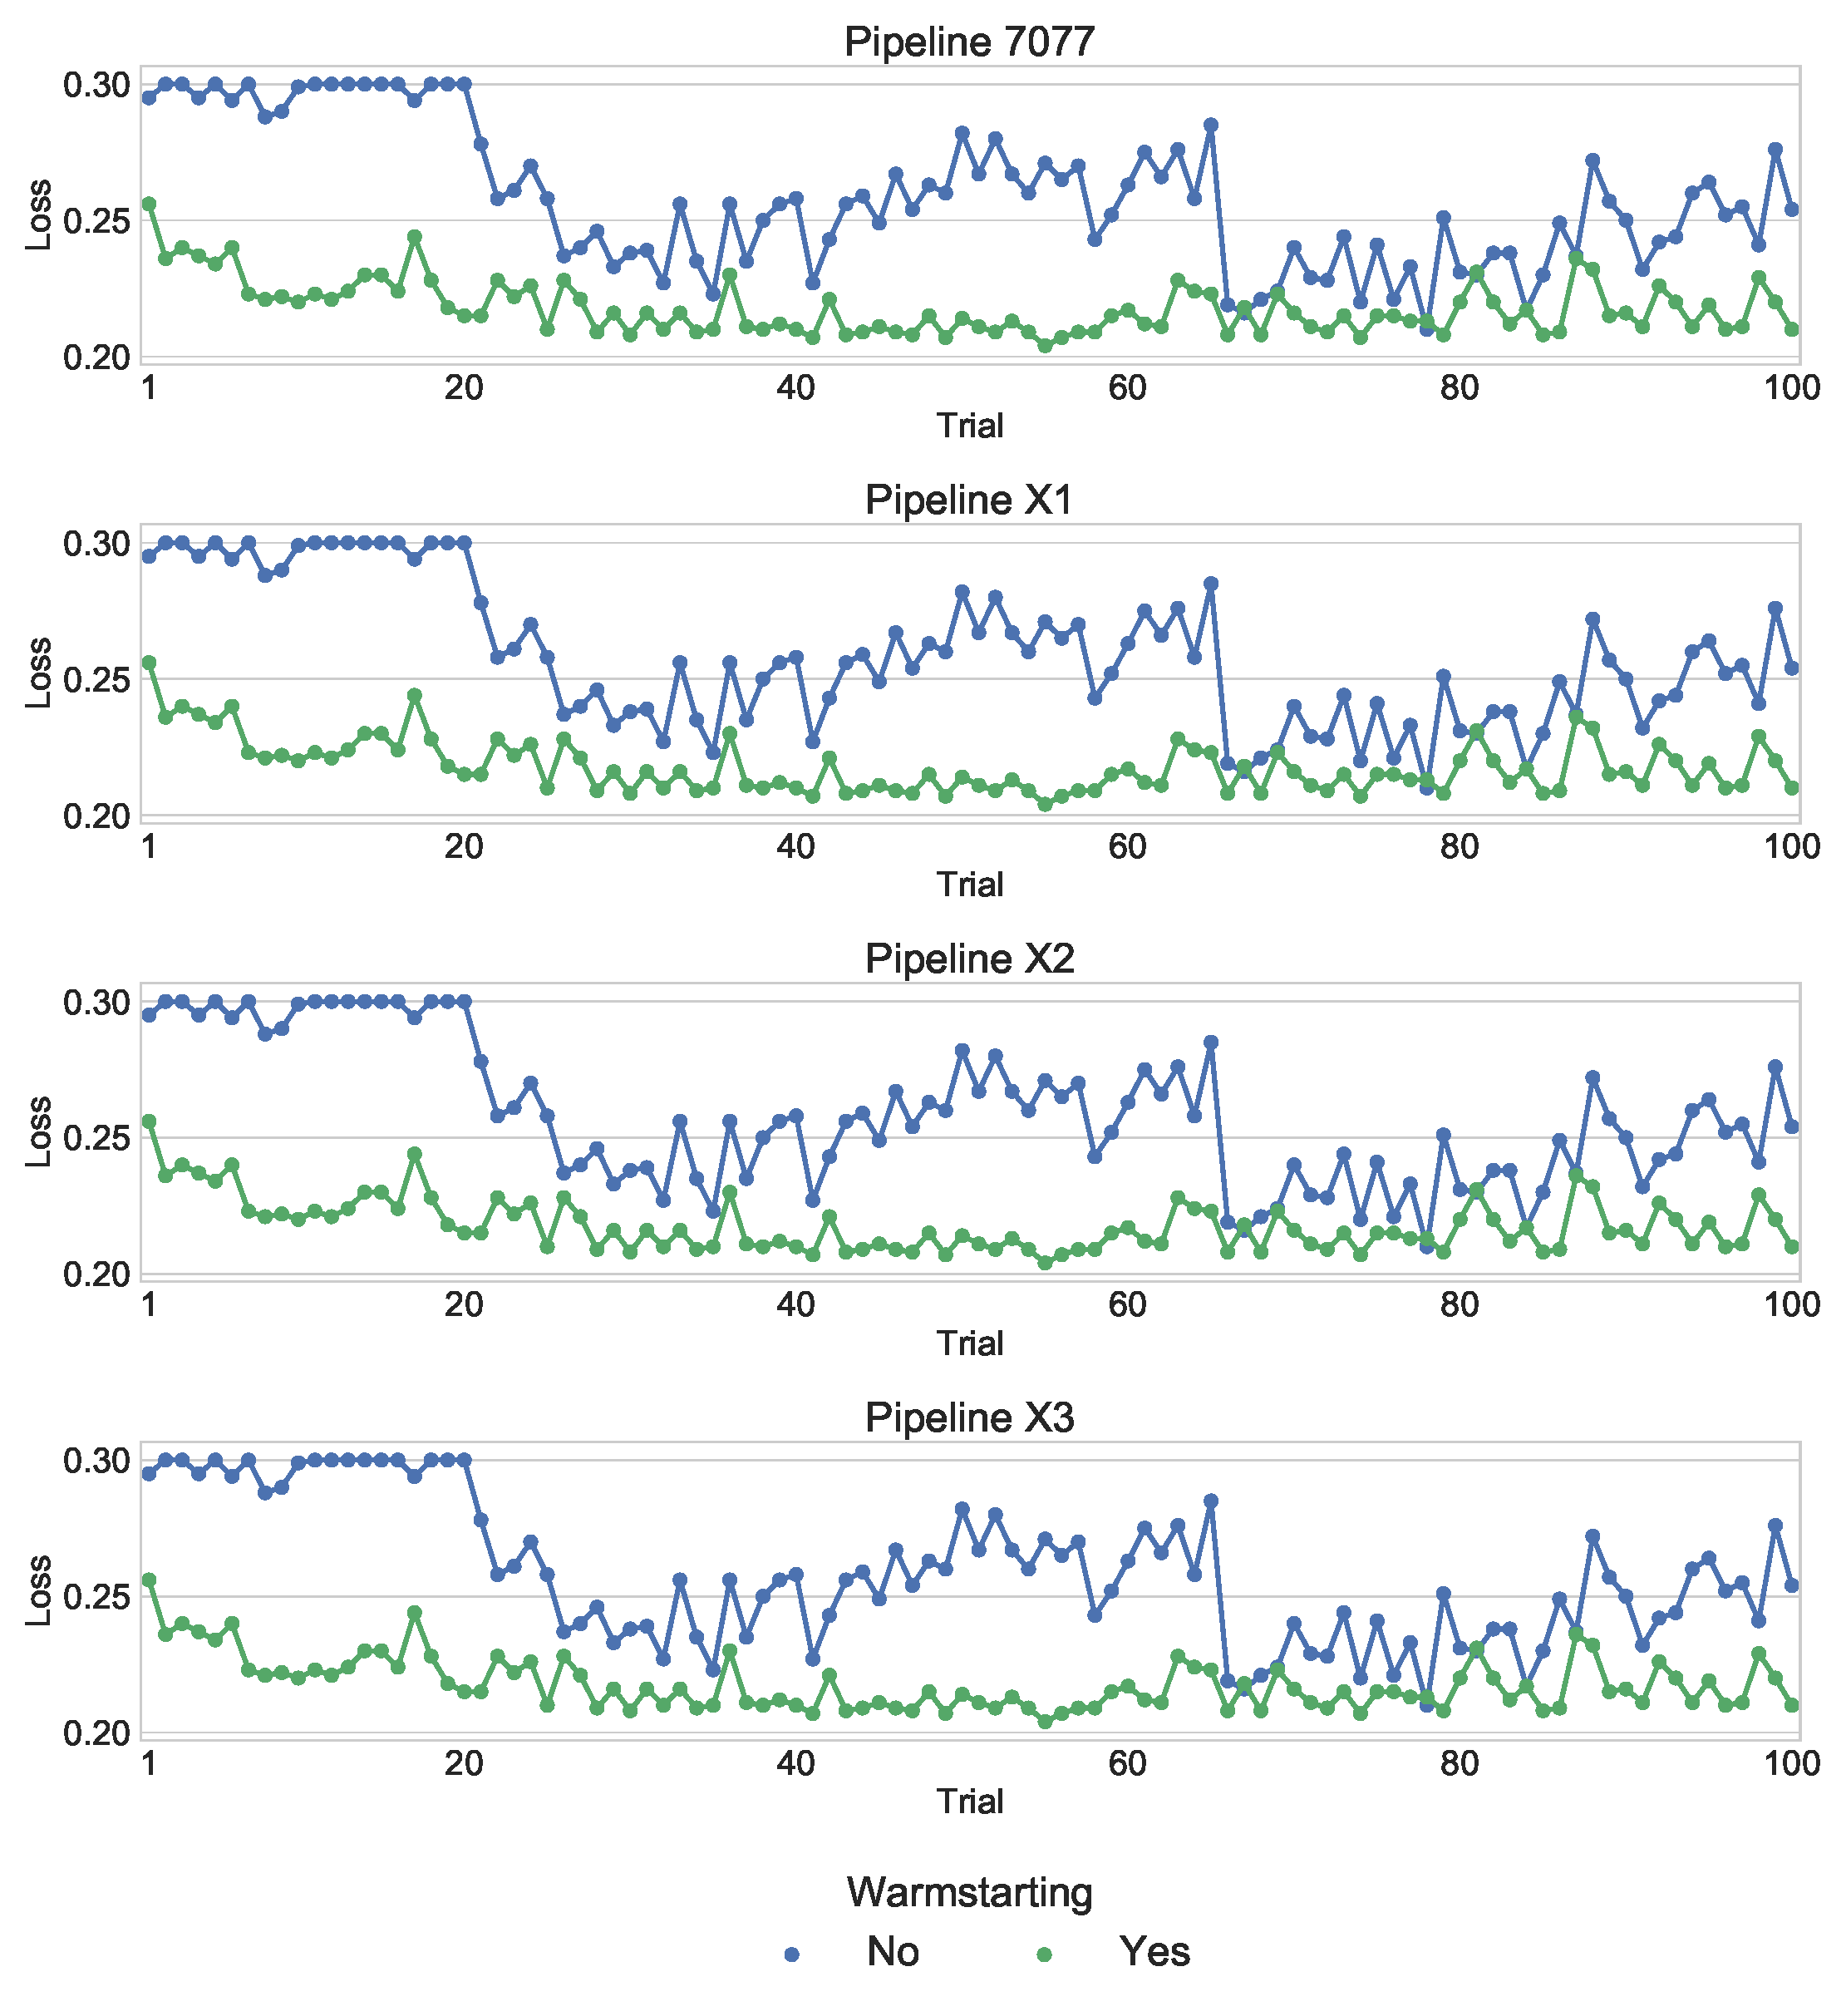
\includegraphics[width=\columnwidth]{../images/experiment-results/task31-cold-starting-warm-avgtrials.eps}
\caption{Loss value of 100 Trials with and without warmstarting}
\label{fig-avg-warm-vs-cold-task-31}
\end{figure}

Table \ref{table-best-hyperparameters} shows the best loss achieved from the search process for every pipeline on the Task 31.
Figure \ref{figure-best-hyperparameters} shows the number of time that the search process (with budget of 100) manages to find the best set of hyperparameters that results in the lowest loss value.
While both with and without warm starting does find the best set of hyperparameters, using warmstarting outperforms the search without wamrstarting and has a higher probability of finding the best hyperparameters.

\begin{minipage}{\columnwidth}
  \begin{minipage}[m]{0.49\columnwidth}
   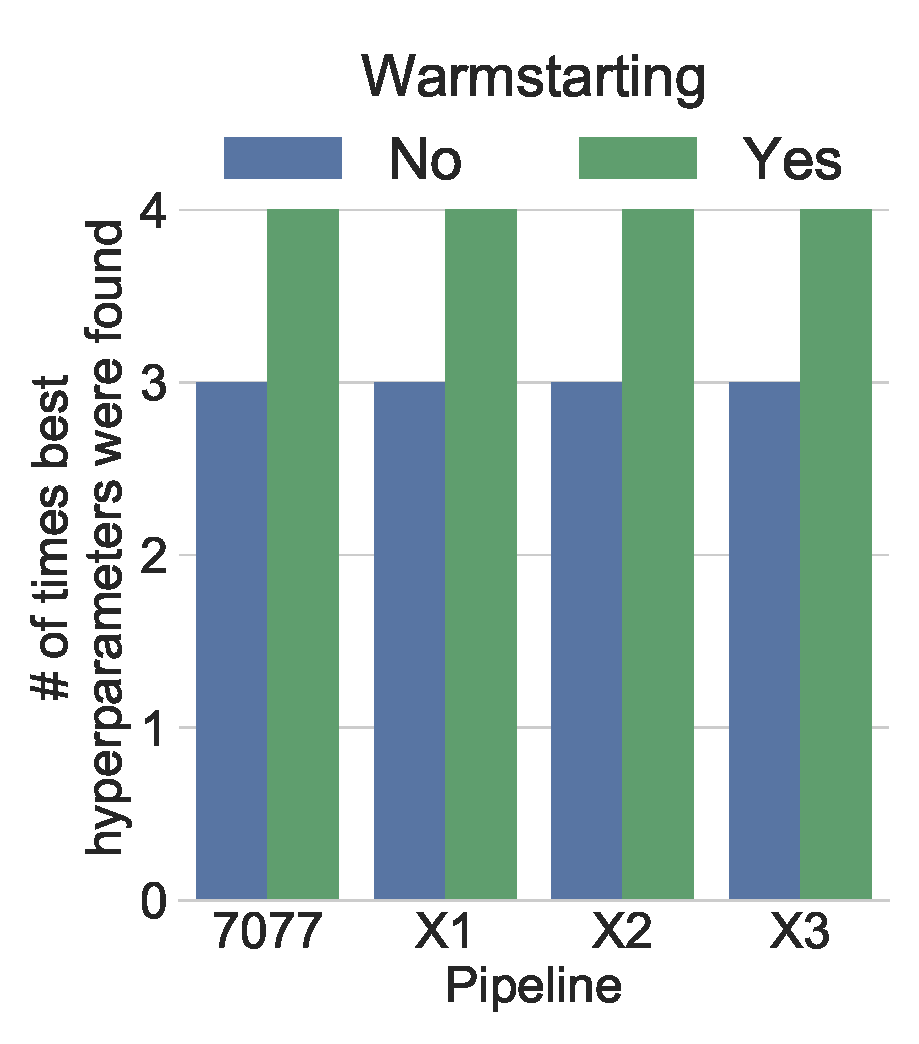
\includegraphics[width=\columnwidth]{../images/experiment-results/task31-cold-starting-warm-besthyperparametersfound.eps}
    \captionof{figure}{Occurrences of best hyperparameters}
     \label{figure-best-hyperparameters}
  \end{minipage}
  \hspace{0.5cm}
  \begin{minipage}[m]{0.49\columnwidth}
    \begin{tabular}{cc}\hline
      Pipeline & Best Loss \\ \hline
        7077 & 0.189 \\
        X1 & XXX \\
        X2 & XXX \\
        X3 & XXX\\ \hline
      \end{tabular}
      \captionof{table}{Best hyperparameters}
      \label{table-best-hyperparameters}
    \end{minipage}
  \end{minipage}
\subsection{Data Materialization}
\section{Related Work} \label{sec-related-work}
Our system lies at the intersection of 3 categories of existing work.
The first category consists of data science platforms that enable collaboration between users.
The second category is data management and provenance systems that capture the relationship between data artifacts.
The last category contains ML and database systems that optimize workloads through materialization and reuse.

\textbf{Collaborative Data Science Platforms.}
Cloud-based systems, such AzureML \cite{team2016azureml}, Google's AI platform \cite{googleai}, Kaggle \cite{kagglewebsite}, and Google Colaboratory \cite{googlecolab} provide the necessary tools for users to write ML workloads in Jupyter notebooks.
Furthermore, users can publish and share their notebooks with others, which could result in higher quality workloads.
However, none of these systems manage the generated ML artifacts and do not utilize them to optimize the execution of the workloads.
Our system manages the ML artifacts and offers reuse and warmstarting methods to decrease the execution time of the future workloads.

OpenML \cite{vanschoren2014openml}, ModelDB \cite{vartak2016m}, and MLflow \cite{zaharia2018accelerating} are platforms that store ML artifacts, such as models and intermediate datasets, in a database \cite{schelter2017automatically, Vanschoren2012}.
These platforms provide APIs for users to query the details of the ML artifacts.
Contrary to our systems, none of these platforms offer automatic materialization and reuse of the ML artifacts.

\textbf{Data Management and Provenance.}
DataHub \cite{bhardwaj2014datahub, bhattacherjee2015principles}, Context \cite{garcia2018context}, Ground \cite{hellerstein2017ground}, ProvDB \cite{miao2018provdb}, Aurum \cite{fernandez2018aurum}, and JuNEAU \cite{ives2019dataset} are data management and provenance systems that efficiently store fine-grained lineage information about the data artifacts and operations.
% Furthermore, some of these systems provide primitives for querying lineage and discovering datasets.
We design our Experiment Graph by utilizing the approaches discussed in these systems.
Specifically, we follow DataHub's graph representation.
However, contrary to these systems, we utilize the stored information to optimize the execution of the workloads.
Our materialization algorithm extends the materialization approach of Bhattacherjee et al. \cite{bhattacherjee2015principles} to tailor it to ML workloads by considering the quality of the model artifacts.

\textbf{Materialization and Reuse in ML and Databases.}
View selection is a long-studied problem in databases, which concerns itself with finding an appropriate set of views to materialize to speed up the execution of queries \cite{mami2012survey}.
Several ML systems utilize such techniques to optimize the execution of workloads. 
Helix \cite{xin2018h, xin2018helix}, DeepDive \cite{zhang2015deepdive}, Columbus \cite{zhang2016materialization}, KeystoneML \cite{sparks2017keystoneml}, and Mistique \cite{vartak2018mistique} are ML systems which optimize workloads by materializing intermediate data for reuse.
These systems have three fundamental differences with our system.
First, the workload DAGs are typically small as these systems work with small ML pipelines.
Therefore, these systems do not need to tackle the problem of searching for reuse opportunities in a large graph.
Helix is the only system that offers a polynomial-time reuse algorithm, which has a higher overhead when compared to our linear-time reuse algorithm.
Second, the materialization decisions in these systems only utilize run-time and size and do not take into account the model quality.
Third, our system operates in a collaborative and multi-tenant environment.
Whereas, the scope of optimization in these systems, except for Mistique, is limited to a single session.
However, Mistique is a model diagnosis tool, which enables users to query intermediate artifacts from an artifact store efficiently.
Whereas, we focus on generating optimal execution plans for future workloads by reusing the artifacts in EG.
Nectar \cite{gunda2010nectar} and ReStore \cite{elghandour2012restore} offer materialization and reuse of intermediate data generated in DryadLINQ \cite{fetterly2009dryadlinq} and MapReduce jobs.
However, Both of these systems only support simple data processing pipelines and do not offer any optimizations for ML workloads.
\section{Conclusions} \label{sec-conclusion}
We present a system for optimizing machine learning workloads in collaborative environments.
We propose a graph representation of the artifacts of ML workloads, which we refer to as the Experiment Graph.
Using the Experiment Graph, we offer materialization and reuse algorithms.
We propose two materialization algorithms.
The first algorithm stores artifacts of the graph based on their likelihood of reappearing in future workloads.
The second algorithm is storage-aware, i.e., it takes deduplication information of the artifacts into account.
Given the set of materialized artifacts, for a new workload, our reuse algorithm finds the optimal execution plan in linear time.

We show that our collaborative optimizer improves the execution time of ML workloads by more than one order of magnitude for repeated executions and by 50\% for modified workloads.
In a real collaborative environment, where users re-execute and modify thousands of workloads, this amounts to hundreds to thousands of hours of execution time saved.
There is considerable overlap in intermediate datasets of ML workload.
As a result, our storage-aware materialization algorithm stores up to 8 times more artifacts than the simple materialization algorithm.
Lastly, our reuse algorithm finds the optimal execution plan and outperforms two baselines, i.e., loading all materialized vertices and recomputing all the vertices.

\textbf{Future work.}
Many data transformation in ML workloads are commutative, i.e., changing the order does not have an impact on the final result.
Currently, we reuse artifacts from EG only when they have the same preceding operations (in the same order) and ignore the commutative property of the operations.
IIn future work, we plan to exploit such transformations and define the concept of DAG equality in the presence of commutative operations.
Furthermore, EG contains valuable information about the meta-data and hyperparameters of the data preprocessing, feature engineering, and model training operations.
In future work, we plan to utilize this information to perform automatic ML pipeline construction and hyperparameter tuning \cite{Feurer15, thornton2013auto}.
Thus, fully or partially automating the process of designing ML pipelines.




\bibliographystyle{abbrv}
\bibliography{references}
\end{document}